%%%%%%%%%%%%%%%%%%%%%%%%%%%%%%%%%%%%%%%%%
%%%%%%%%%%%%%%%%%%%%%%%%%%%%%%%%%%%%%%%%%
% Beamer Presentation
% LaTeX Template
% Version 1.0 (10/11/12)
%
% This template has been downloaded from:
% http://www.LaTeXTemplates.com
%
% License:
% CC BY-NC-SA 3.0 (http://creativecommons.org/licenses/by-nc-sa/3.0/)
%
%%%%%%%%%%%%%%%%%%%%%%%%%%%%%%%%%%%%%%%%%

%----------------------------------------------------------------------------------------
%	PACKAGES AND THEMES
%----------------------------------------------------------------------------------------

\documentclass{beamer}

\mode<presentation> {

% The Beamer class comes with a number of default slide themes
% which change the colors and layouts of slides. Below this is a list
% of all the themes, uncomment each in turn to see what they look like.

%\usetheme{default}
%\usetheme{AnnArbor}
%\usetheme{Antibes}
%\usetheme{Bergen}
%\usetheme{Berkeley}
%\usetheme{Berlin}
%\usetheme{Boadilla}
%\usetheme{CambridgeUS}
%\usetheme{Copenhagen}
%\usetheme{Darmstadt}
%\usetheme{Dresden}
%\usetheme{Frankfurt}
%\usetheme{Goettingen}
%\usetheme{Hannover}
%\usetheme{Ilmenau}
%\usetheme{JuanLesPins}
%\usetheme{Luebeck}
\usetheme{Madrid}
\usepackage{tcolorbox}
\usepackage{amsmath,amssymb}
\usepackage{proof}
\usepackage{bbm}
\usepackage{ulem}
\usepackage{tikz}
\usepackage{tikz-cd}
\newcommand{\vp}{\vspace*{5pt}}
\newcommand{\tr}{\text{ is true}}
\newcommand{\pp}{\text{ is prop}}
\newcommand{\trx}{\text{ tr}}
%\usetheme{Malmoe}
%\usetheme{Marburg}
%\usetheme{Montpellier}
%\usetheme{PaloAlto}
%\usetheme{Pittsburgh}
%\usetheme{Rochester}
%\usetheme{Singapore}
%\usetheme{Szeged}
%\usetheme{Warsaw}

% As well as themes, the Beamer class has a number of color themes
% for any slide theme. Uncomment each of these in turn to see how it
% changes the colors of your current slide theme.

%\usecolortheme{albatross}
%\usecolortheme{beaver}
%\usecolortheme{beetle}
%\usecolortheme{crane}
%\usecolortheme{dolphin}
%\usecolortheme{dove}
%\usecolortheme{fly}
%\usecolortheme{lily}
%\usecolortheme{orchid}
%\usecolortheme{rose}
%\usecolortheme{seagull}
%\usecolortheme{seahorse}
%\usecolortheme{whale}
%\usecolortheme{wolverine}

%\setbeamertemplate{footline} % To remove the footer line in all slides uncomment this line
%\setbeamertemplate{footline}[page number] % To replace the footer line in all slides with a simple slide count uncomment this line

%\setbeamertemplate{navigation symbols}{} % To remove the navigation symbols from the bottom of all slides uncomment this line
}


\usepackage{xcolor}
\usepackage{stmaryrd}
\usepackage{tikz}
\usepackage{tikz-cd}
\usetikzlibrary{matrix,arrows,decorations.pathmorphing}
\definecolor{red}{rgb}{1,0,0}
\usepackage{gensymb}
\usepackage{graphicx} % Allows including images
\usepackage{booktabs} % Allows the use of \toprule, \midrule and \bottomrule in tables
\usepackage{verbatim}


%----------------------------------------------------------------------------------------
%	TITLE PAGE
%----------------------------------------------------------------------------------------

\title[Theorem Proving]{Theorem Proving in Haskell} % The short title appears at the bottom of every slide, the full title is only on the title page
\subtitle{CIS 552 Project}

\author[Choudhury \& Li]{Pritam Choudhury and Yao Li} % Your name
\institute[] % Your institution as it will appear on the bottom of every slide, may be shorthand to save space
{
Department of Computer and Information Science\\ % Your institution for the title page
\medskip
{University of Pennsylvania} % Your email address
}
\date{\today} % Date, can be changed to a custom date

\begin{document}

\begin{frame}
\titlepage % Print the title page as the first slide
\end{frame}

%\begin{frame}
%\frametitle{Overview} % Table of contents slide, comment this block out to remove it
%\tableofcontents % Throughout your presentation, if you choose to use \section{} and \subsection{} commands, these will automatically be printed on this slide as an overview of your presentation
%\end{frame}

%----------------------------------------------------------------------------------------
%	PRESENTATION SLIDES
%----------------------------------------------------------------------------------------

%------------------------------------------------
 % Sections can be created in order to organize your presentation into discrete blocks, all sections and subsections are automatically printed in the table of contents as an overview of the talk
%------------------------------------------------

 % A subsection can be created just before a set of slides with a common theme to further break down your presentation into chunks
\begin{frame}
\frametitle{\centerline{Natural Deduction Style (Selected Rules)}}
$$\infer[(\wedge \text{I})]{\Gamma \vdash \phi_1 \wedge \phi_2 }{\Gamma \vdash \phi_1 & \Gamma \vdash \phi_2}$$ \vp 
$$ \infer[(\wedge \text{E}1)]{\Gamma \vdash \phi_1}{\Gamma \vdash \phi_1 \wedge \phi_2}$$ \vp
$$ \infer[(\wedge \text{E}2)]{\Gamma \vdash \phi_2}{\Gamma \vdash \phi_1 \wedge \phi_2}$$ 

\end{frame}


%------------------------------------------------
\begin{frame}
\frametitle{\centerline{Encoding in Haskell}}
\begin{problem}
 How do we encode these rules of inference in Haskell?
 \end{problem}
 \vp \pause
\begin{itemize}
\item Rules of inference as partial functions on sequents \pause
\item Rules of inference as constructors of an inductive data structure
\end{itemize} 
 
\end{frame}

%-------------------------------------------------------

\begin{frame}
\frametitle{\centerline{Rules as functions on sequents}} 
$$\infer[(\wedge \text{I})]{\Gamma \vdash \phi_1 \wedge \phi_2 }{\Gamma \vdash \phi_1 & \Gamma \vdash \phi_2}$$ \vp 
\centerline{\texttt{andI :: Sequent -> Sequent -> Maybe Sequent}} \pause
$$\infer[(\vee \text{I}1)]{\Gamma \vdash \phi_1 \vee \phi_2}{\Gamma \vdash \phi_1}$$ \vp 
\centerline{\texttt{orI1 :: Formula -> Sequent -> Maybe Sequent}}  \pause 
\begin{equation*}
\phi_1 \wedge (\phi_2 \vee \phi_3) \vdash (\phi_1 \wedge \phi_2) \vee (\phi_1 \wedge \phi_3)
\end{equation*}
\centerline{\texttt{distr :: Formula -> Formula -> Formula -> Maybe Sequent}}
\end{frame}

%--------------------------------------------------------

\begin{frame}
\frametitle{\centerline{In Kind Formula}}
\centerline{\texttt{distr :: Derives '[And p (Or q r)] ->}} \centerline{\texttt{(Or (And p q) (And p r))}}
\pause \vspace*{20pt}

\centerline{\texttt{OrI1 :: Derives ctx p -> Derives ctx (Or p q)}} \pause \vspace*{20pt}

\center{\texttt{AndI :: Derives ctx p -> \\
                        \hspace*{45pt}    Derives ctx q -> \\ 
                         \hspace{74pt}   Derives ctx (And p q)}}

\end{frame}
 
 %------------------------------------------------------------

\begin{frame}
\frametitle{\centerline{Printing Proof-Trees}}

"Add information about singleton types and other printing functions."

\end{frame}


%--------------------------------------------------------

\begin{frame}
\frametitle{\centerline{Populating the formulas}}
\begin{center}
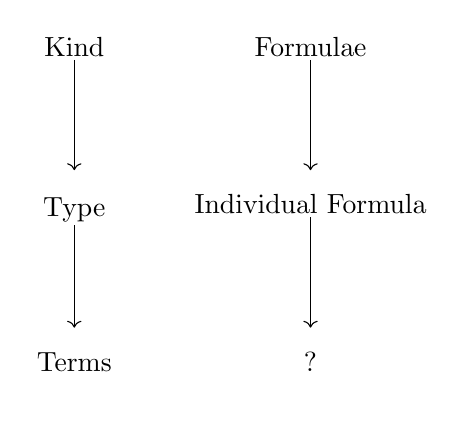
\begin{tikzpicture}

    \node[label={Formulae}] (a1) at (3,4) {};
    \node[label={Individual Formula}] (a2) at (3,2) {};
    \node[label={?}] (a3) at (3,0) {};
    \node[label={Kind}] (b1) at (0,4) {};
    \node[label={Type}] (b2) at (0,1.9) {};
    \node[label={Terms}] (b3) at (0,0) {};
        
    \draw[->] (3,4.2) -- node[above]{} (3,2.8);
    \draw[->] (3,2.2) -- node[right]{} (3,0.8);
    \draw[->] (0,4.2) -- node[left]{} (0,2.8);
    \draw[->] (0,2.1) -- node[below]{} (0,0.8);
    
\end{tikzpicture}
\end{center} 
\end{frame}

%----------------------------------------------------------

\begin{frame}
\frametitle{\centerline{Formula as Type Constructor}}
\begin{center}
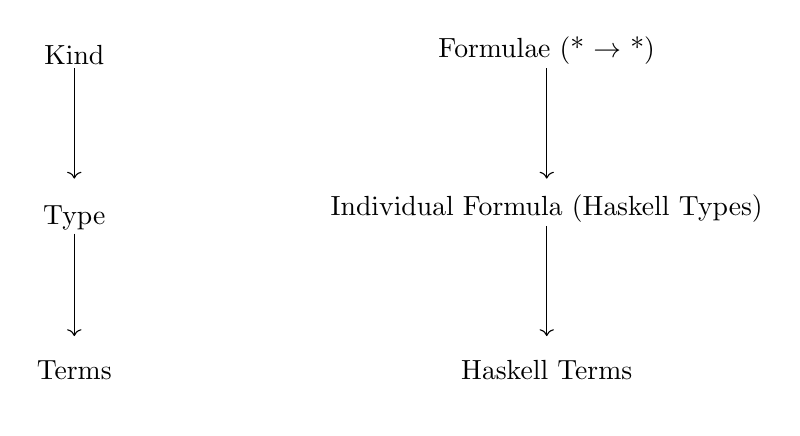
\begin{tikzpicture}

    \node[label={Formulae (* $\to$ *)}] (a1) at (6,4) {};
    \node[label={Individual Formula (Haskell Types)}] (a2) at (6,2) {};
    \node[label={Haskell Terms}] (a3) at (6,0) {};
    \node[label={Kind}] (b1) at (0,4) {};
    \node[label={Type}] (b2) at (0,1.9) {};
    \node[label={Terms}] (b3) at (0,0) {};
        
    \draw[->] (6,4.2) -- node[above]{} (6,2.8);
    \draw[->] (6,2.2) -- node[right]{} (6,0.8);
    \draw[->] (0,4.2) -- node[left]{} (0,2.8);
    \draw[->] (0,2.1) -- node[below]{} (0,0.8);
    
\end{tikzpicture}
\end{center} 
\end{frame}

%---------------------------------------------------------------

\begin{frame}
\frametitle{\centerline{Derivation and Evidence in one go}}
\centerline{\texttt{distrD :: Derives '[Formula (p :$\wedge$: (q :$\vee$: r))]}}

\centerline{\texttt{(Formula ((p :$\wedge$: q) :$\vee$: (p :$\wedge$: r)))}}
\vspace*{20pt}
\centerline{\texttt{distrE :: Evidence '[Formula (p :$\wedge$: (q :$\vee$: r))]}}

\centerline{\texttt{(Formula ((p :$\wedge$: q) :$\vee$: (p :$\wedge$: r)))}}
\pause
\vspace{20pt}
\begin{itemize}
\item Derivation using just the rules of inference \vspace{20pt}
\item Evidence by looking inside the types
\end{itemize}
\end{frame}

%---------------------------------------------------------

\begin{frame}[fragile]
\frametitle{\centerline{Tracking the Proof-Objects}}
\begin{align*}
x : p \wedge (q \vee r) \vdash \text{ case } & (\text{snd } x) \\
                          \{ & x1 \to i1 \text{ }(\text{fst } x, x1) \text{ } |  \\
                            & x2 \to i2 \text{ }(\text{fst } x, x2) \} : (p \wedge q) \vee (p \wedge r)
\end{align*}

 \pause
 \vspace*{20pt}
 
\begin{verbatim}
 distrP :: Derives '[IsProof x (p :/\: (q :\/: r))]
                      (Case (Proj2 x) 
                         x1 (Inj1 (Pair (Proj1 x) x1))
                         x2 (Inj2 (Pair (Proj1 x) x2)))
                      (Formula ((p :/\: q) :\/: (p :/\: r)))
\end{verbatim} 



\end{frame}

%---------------------------------------------------------

\begin{frame}
\frametitle{\centerline{Derivation provides evidence of its derivant}} 
\center{\texttt{Derives ctx (Formula a) $\to$ Evidence ctx (Formula a)}}
\end{frame}

%-------------------------------------------------------------------------------------------

\begin{frame}
\Huge{\centerline{Questions?}}
\end{frame}

%-------------------------------------------------------------------------------------------

\begin{frame}
\begin{tcolorbox}[colback=green!5,colframe=green!40!black]
\Huge{\centerline{Thank you.}}
\end{tcolorbox}
\end{frame}

%------------------------------------------------------------------------------------------

\end{document}
